\documentclass[runningheads,a4paper]{llncs}

\usepackage{amssymb}
\setcounter{tocdepth}{3}

\usepackage{graphicx}

\usepackage{url}

\urldef{\mailsa}\path|alexa.schlegel@gmail.com|
\newcommand{\keywords}[1]{\par\addvspace\baselineskip
\noindent\keywordname\enspace\ignorespaces#1}

\renewcommand*\familydefault{\sfdefault}

\usepackage{xcolor}
\definecolor{usethiscolorhere}{rgb}{0.85,0.85,0.85}

\begin{document}

\mainmatter  % start of an individual contribution

% first the title is needed
\title{Temporal Development of Overlapping Communities in Co-Authorship Networks}

% a short form should be given in case it is too long for the running head
\titlerunning{Temporal Development of Overlapping Communities}

% the name(s) of the author(s) follow(s) next
%
% NB: Chinese authors should write their first names(s) in front of
% their surnames. This ensures that the names appear correctly in
% the running heads and the author index.
%
\author{Alexa Schlegel%
}
%
\authorrunning{Temporal Development of Overlapping Communities}
% (feature abused for this document to repeat the title also on left hand pages)

% the affiliations are given next; don't give your e-mail address
% unless you accept that it will be published
\institute{Freie Universit{\"a}t Berlin, Institute of Computer Science\\
\mailsa\\
}

%
% NB: a more complex sample for affiliations and the mapping to the
% corresponding authors can be found in the file "llncs.dem"
% (search for the string "\mainmatter" where a contribution starts).
% "llncs.dem" accompanies the document class "llncs.cls".
%

\toctitle{Temporal Development of Overlapping Communities in Co-Authorship Networks}
\maketitle


\begin{abstract}
Detection of overlapping communities plays an important role when it comes to analysing scientific collaboration using social networks. The present paper describes a method to analyse the temporal development of overlapping communities within co-authorship networks. The paper mainly relies on the clique percolation method for community extraction. propounded by Palla~et~al. The main goal is to find and understand an appropriate algorithm, that can be applied to an existing dataset of scientific publications. Implications for further actions and time complexity are discussed.

\keywords{co-authorship networks, scientific collaboration networks, overlapping community detection, temporal analysis, clique percolation, dynamic communities}
\end{abstract}

\section{Introduction and Motivation}
A \emph{social network} is a representation of a social structure comprising actors such as individuals, affiliations, as well as their social interactions.
The network model conceptualizes social, economic, or political structures as lasting patterns of interactions between actors.~\cite{wasserman1994social}

A \emph{co-authorship network} is a scientific collaboration network, with scientists as actors, where the social interaction leads to collaborative papers.
In mathematical terms, networks are graphs, and thus consist of nodes (vertex) and links (edges).
In a co-authorship network, nodes are individual authors who are considered connected if they co-author a paper.~\cite{newman2001structure}

Usually, those networks are used to study patterns of scientific collaboration in different fields, their development over time, identify key people regarding different network measurements, detection and evolution of communities, and more. See~\cite{barabasi2002evolution}, \cite{newman2001structure} and \cite{newman2004coauthorship} for more details.

This seminar paper is motivated by a dataset of $2.277$ publications related to geochemistry focusing on papers talking about stable metal isotopes (e.g.~potassium, magnesium, lithium, silicon, etc.). This data was used to build a cumulated co-authorship network using a simple approach to model collaboration.

The dataset was collected using the bibliographic database scopus\footnote{\url{http://www.scopus.com/}, accessed: March 2014} and includes publications starting from 1997/98 until 2014.
The dataset comprised of authors, co-authors, title, year, abstract and affiliations.
A basic network analysis has already been performed regarding such aspects as centrality measurement, community detection, degree distribution, and average degree.

Since the dataset includes temporal information~(publishing year), the following question arises: How do communities within this type of co-authorship network evolve over time? In geochemistry, people often tend to focus on one isotope system and stick to this topic for a long time. Do researchers in geochemistry really focus on one specific topic or change the field over time?

Therefore, this seminar paper aims is to find and explain an already established and well-understood method for analysing the temporal development of communities within co-authorship networks. The main point is to understand the underlying algorithm in detail, and to find out implications and challenges when applying this method to the geochemistry dataset.

\section{Related Work}
\label{related}
The related work focuses on algorithms for community detection especially for co-authorship networks and seeks to track those detected communities over time.
``Most real world networks contain parts in which nodes are more highly connected to each other than to the rest of the network, those sets are usually called clusters, communities, cohesive groups or modules, they have no widely accepted, unique definition.''~\cite{palla2005uncovering}
The precision with which ``more highly connected'' is defined makes the difference between community detection algorithms.
It depends on the heuristic that is employed to identify communities.~\cite{porter2009communities}

Fortunato~\cite{fortunato2010community} gives an extended overview of the various types of community detection algorithms.
Explaining any of those would be beyond the scope of this work.
For example, traditional methods include algorithms based on graph partitioning, hierarchical clustering, and spectral clustering.
There are also divisive and agglomerative algorithms.
The best-known one from this category is Girvan and Newman~\cite{girvan2002community}.

Most algorithms determine distinctive sets of communities, so a node can only belong to a single community. Most realworld networks consist of overlapping and nested communities, e.g.~friendship network of a person~\cite{palla2005uncovering}.
Fortunato~\cite{fortunato2010community} also gives an overview of algorithms detecting overlapping communities.
The best known and widely cited of these is the \emph{clique percolation method (CPM)} by Palla et~al.~\cite{palla2005uncovering}.
There is an implementation provided by the authors, called \emph{CFinder}\footnote{CFinder is a tool that implements the clique percolation method by Palla. It finds and visualizes overlapping dense groups of nodes in networks. \url{http://www.cfinder.org/}, accessed: 05.12.2015}, as well as one in the R igraph library\footnote{\url{http://igraph.wikidot.com/community-detection-in-r#toc0}, accessed: 05.12.2015}.

Not only do overlapping communities exist in networks, but communities are also structured in a hierarchical manner.
Recent work on algorithms detecting hierarchicla and overlapping structures  include~\cite{1367-2630-11-3-033015}, \cite{Cui201485} and~ \cite{Shen20091706}.

Looking at the temporal development of communities ``the main phenomena occurring in the lifetime of a community are: birth, growth, contraction, merger with other communities, split, death''~\cite{fortunato2010community} (see figure~\ref{fig:evolution}).
The detection of dynamic communities has been studied by Palla et~al.~\cite{palla2007quantifying} using CPM for each snapshot of the graph. Further information on dynamic communities can be found in Section 13 of~\cite{fortunato2010community}.

\begin{figure}
	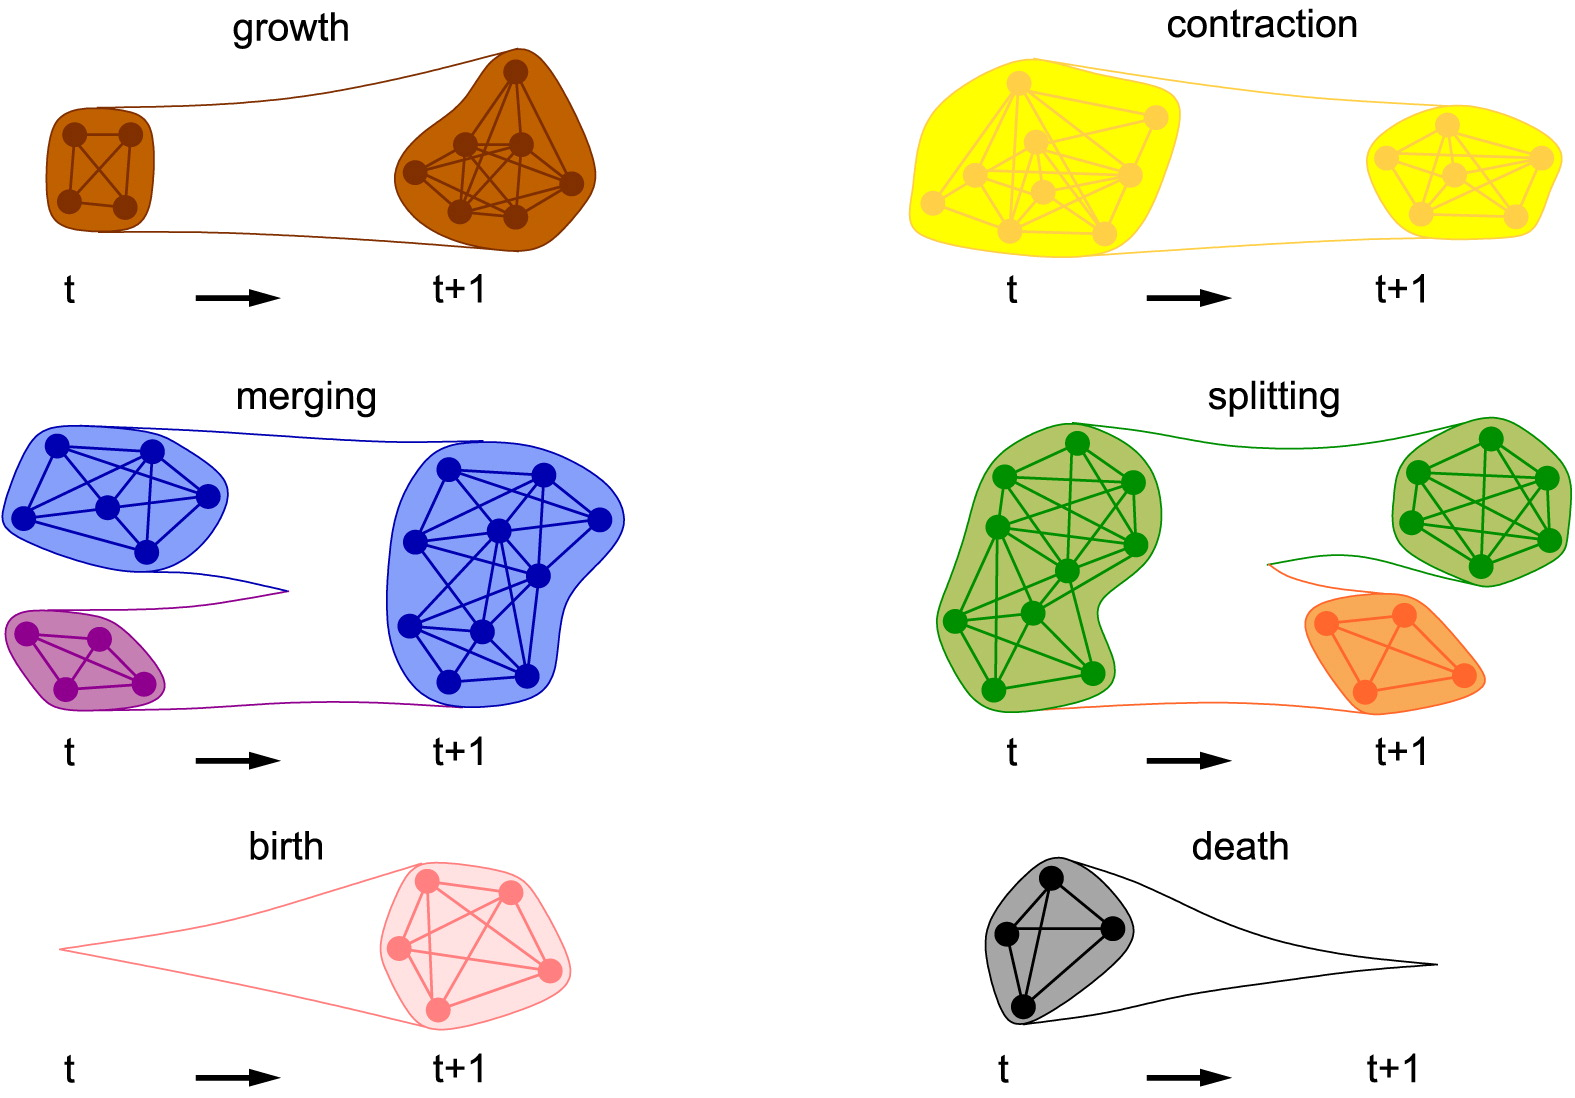
\includegraphics[width=\textwidth]{img/fullSizeEvolution.jpg}
	\caption{Lifetime of a community, from~[9]}
	\label{fig:evolution}
\end{figure}

Since CPM is a widely used method for detecting overlapping communities I will explain this method in more detail. The following sections describe the CPM as wll as the temporal algorithm based on two papers by Palla et~al.~\cite{palla2005uncovering} and~\cite{palla2007quantifying}.

\section{Clique Percolation Method}
\label{cpm}
The clique percolation method (CPM), developed by Palla et~al.~\cite{palla2007quantifying}, is used to identify overlapping communities in unweighted and undirected networks.
The authors tested and evaluated their method using a co-authorship network, protein-protein interaction network, word association networks and a network constructed from variables within the source code of an open-source FTP program.
The following section explains the algorithm and summarizes the main findings of the paper regarding co-authorship networks.

The underlying community definition relies on the fact that a community comprises fully connected subgraphs, called \emph{cliques}.
\emph{$k$-cliques} are fully connected subgraphs with $k$ nodes.
In Figure~\ref{fig:cliques}, an example of $\{3,4\}$-cliques are given.
A community, in this context, is called a \emph{$k$-clique-community}, which is defined as a union of all $k$-cliques, which can be reached from each other through a number of \emph{adjacent $k$-cliques}.
Two $k$-cliques are called adjacent if they share $k-1$ nodes.
In Figure~\ref{fig:rolling}, the so-called $k$-clique template rolling is visualized for a $3$-clique.
A $k$-clique-community is best described by relocating one node until all the nodes of the community are discovered.

\begin{figure}
	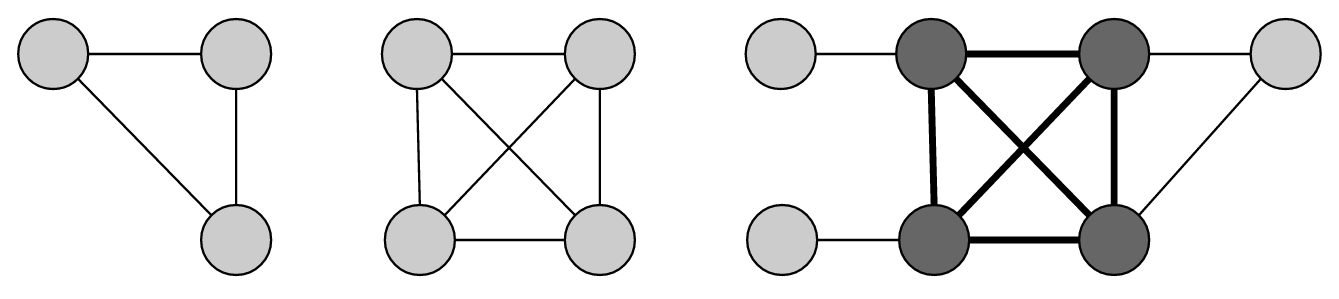
\includegraphics[width=\textwidth]{img/cliques.png}
    \caption{Examples for a $3$-clique, $4$-clique and a $4$-clique inside a graph.}
    \label{fig:cliques}
\end{figure}

\begin{figure}
	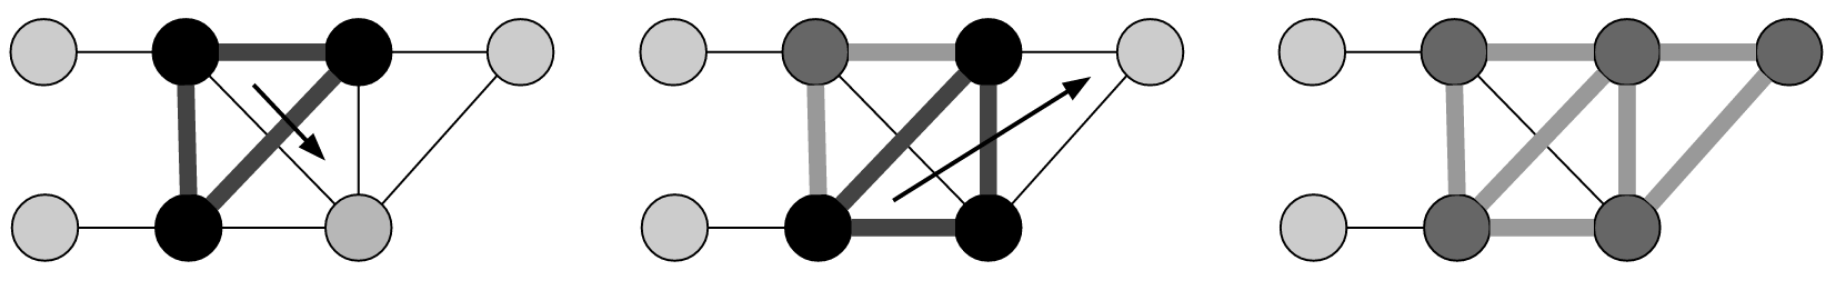
\includegraphics[width=\textwidth]{img/rolling.png}
	\caption{Template rolling for a $3$-clique}
	\label{fig:rolling}
\end{figure}

\subsection{Algorithm}
\label{cpm-algo}
The starting point for the algorithm is an undirected and unweighted graph. In Section \ref{cpm-construction}, we talk about generating the unweighted co-authorship graph.
Based on the explained community definition, the algorithm consists of the following steps:

\medskip

\noindent
\colorbox{usethiscolorhere}{
\begin{minipage}{\dimexpr\textwidth-2\fboxsep}

\begin{enumerate}
\small
\item[(1)] Find all maximal cliques.
\item[(2)] Prepare clique-clique overlap matrix, or clique graph.
\item[(3)] Threshold the matrix with a certain $k$.
\item[(4)] Each connected component in the clique graph forms a $k$-clique-community.
\item[(5)] Post-processing.
\end{enumerate}

\end{minipage}
}

\subsubsection{(1) Find all maximal cliques}
Instead of finding all $k$-cliques, as a first step, the algorithm searches for all maximal cliques. Instead of finding all $k$-cliques, which is a polynomial problem, this can be done in exponential time, state the authors.
Maximal cliques cannot be subsets of larger cliques, which is why they are detected in decreasing order of their size.
The largest possible clique size $s_{max}$ is determined by the maximal degree $d_{max}$ found in the network. The following steps describe the algorithm for finding maximal cliques:

\medskip

\noindent
\colorbox{usethiscolorhere}{
\begin{minipage}{\dimexpr\textwidth-2\fboxsep}

\begin{enumerate}
\small
\item[(1)] Determine $s=s_{max}$.
\item[(2)] Repeatedly choose a node $v$ from the graph:
	\begin{enumerate}
		\item[(2.1)] Extract all cliques of size $s$ containing $v$.
		\item[(2.2)] Delete the node and its edges.
	\end{enumerate}
\item[(3)] When no nodes are left set $s=s-1$ and start with (2) on the original graph.
\end{enumerate}

\end{minipage}
}

\medskip

The set of already found cliques influence the found cliques in later steps, as the later found cliques are smaller.
The detailed algorithm for the step (2.1) to find cliques of size $s$ of $v$ can be looked up in the supplementary material of the paper in Section 1.1.2, page 3.
The result of this step is a set of size $n_c$ containing all maximal cliques, an example of which can be seen in Figure~\ref{fig:allmaxcliques}.

\begin{figure}
\begin{center}
	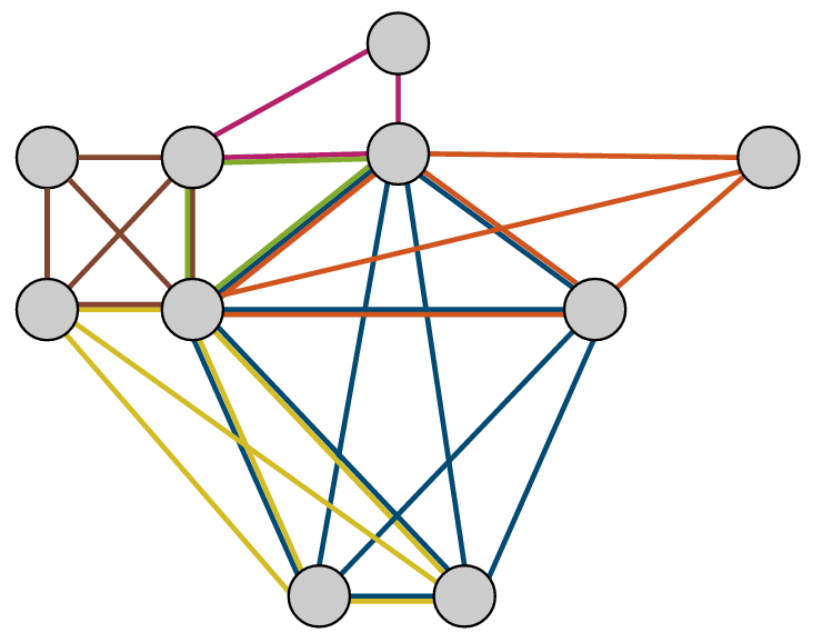
\includegraphics[width=0.8\textwidth]{img/allmaxcliques.png}
		\caption{All maximal cliques in a graph. Each colour represents a maximal clique. Adapted from~[9].}
		\label{fig:allmaxcliques}
\end{center}
\end{figure}

\subsubsection{(2) Prepare clique- clique overlap matrix, or clique graph}
The dimension of the overlap matrix is $n_c \times n_c$.
Each row and column represents a clique.
All non-diagonal matrix elements represent the number of nodes those cliques share.
The diagonal entries represent the size of the corresponding clique.
This matrix is only generated once.
In Figure~\ref{fig:matrix}, the clique- clique overlap matrix of the graph in Figure~\ref{fig:allmaxcliques} and the corresponding clique graph is shown.

\begin{figure}
\begin{center}
	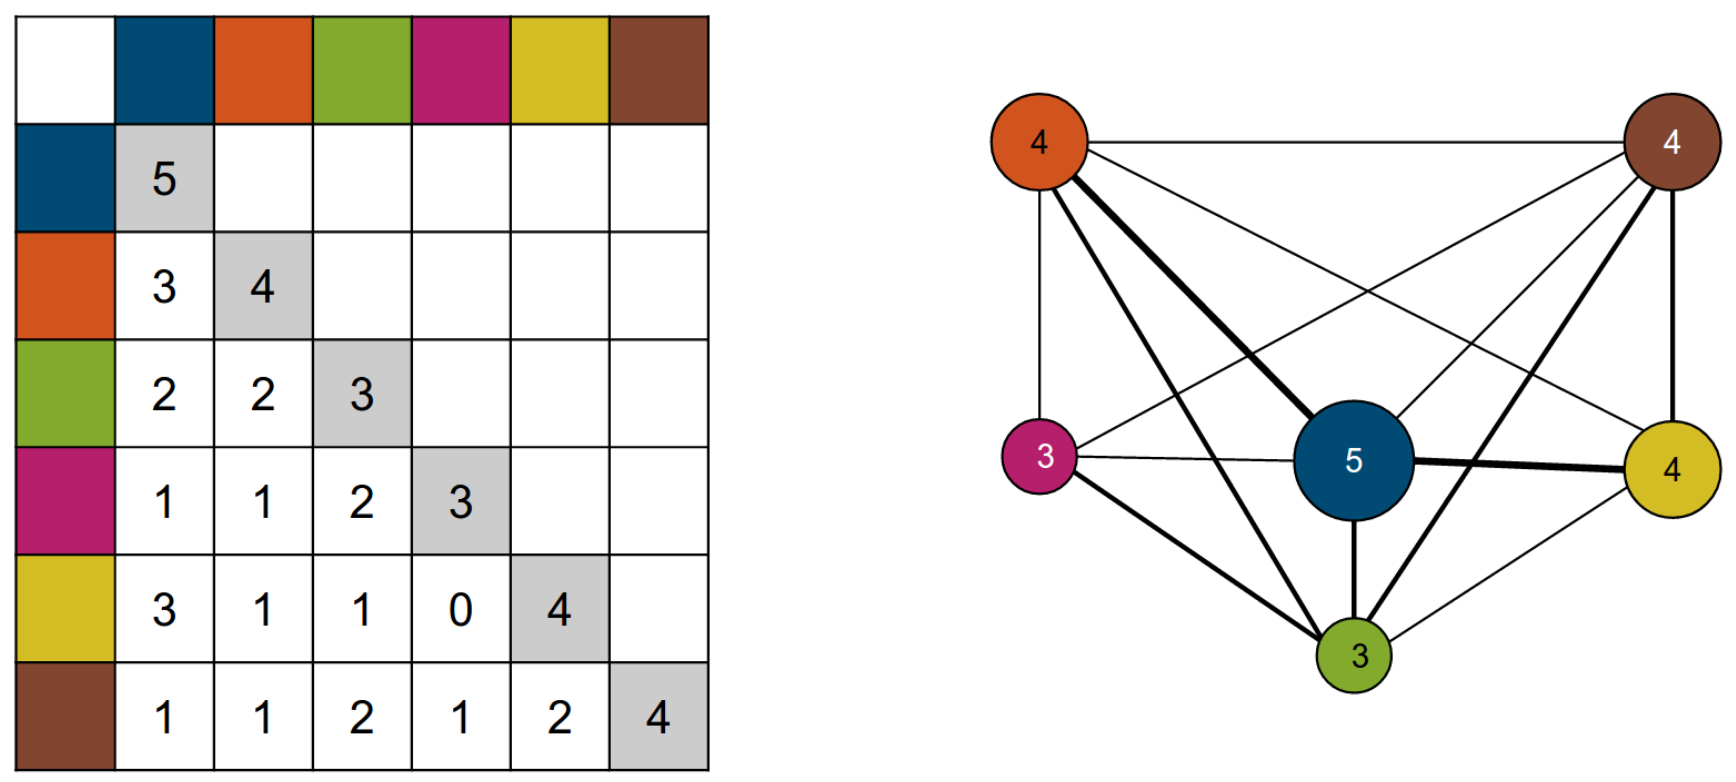
\includegraphics[width=0.8\textwidth]{img/matrix.png}
		\caption{The clique- clique overlap matrix and the corresponding clique graph. The number inside the node is the number of nodes belonging to that community, the width of the edge represents the shared nodes.}
		\label{fig:matrix}
\end{center}		
\end{figure}


\subsubsection{(3) Threshold the matrix}
All off-diagonal entries smaller than $k-1$ and diagonal entries smaller than $k$ are set to $0$.
The remaining elements are set to $1$, resulting in a binary matrix, representing a network of cliques. The thresholding can be done repeatedly without calculating a new matrix. See Figure~\ref{fig:matrixtrashed}.

\begin{figure}
\begin{center}
	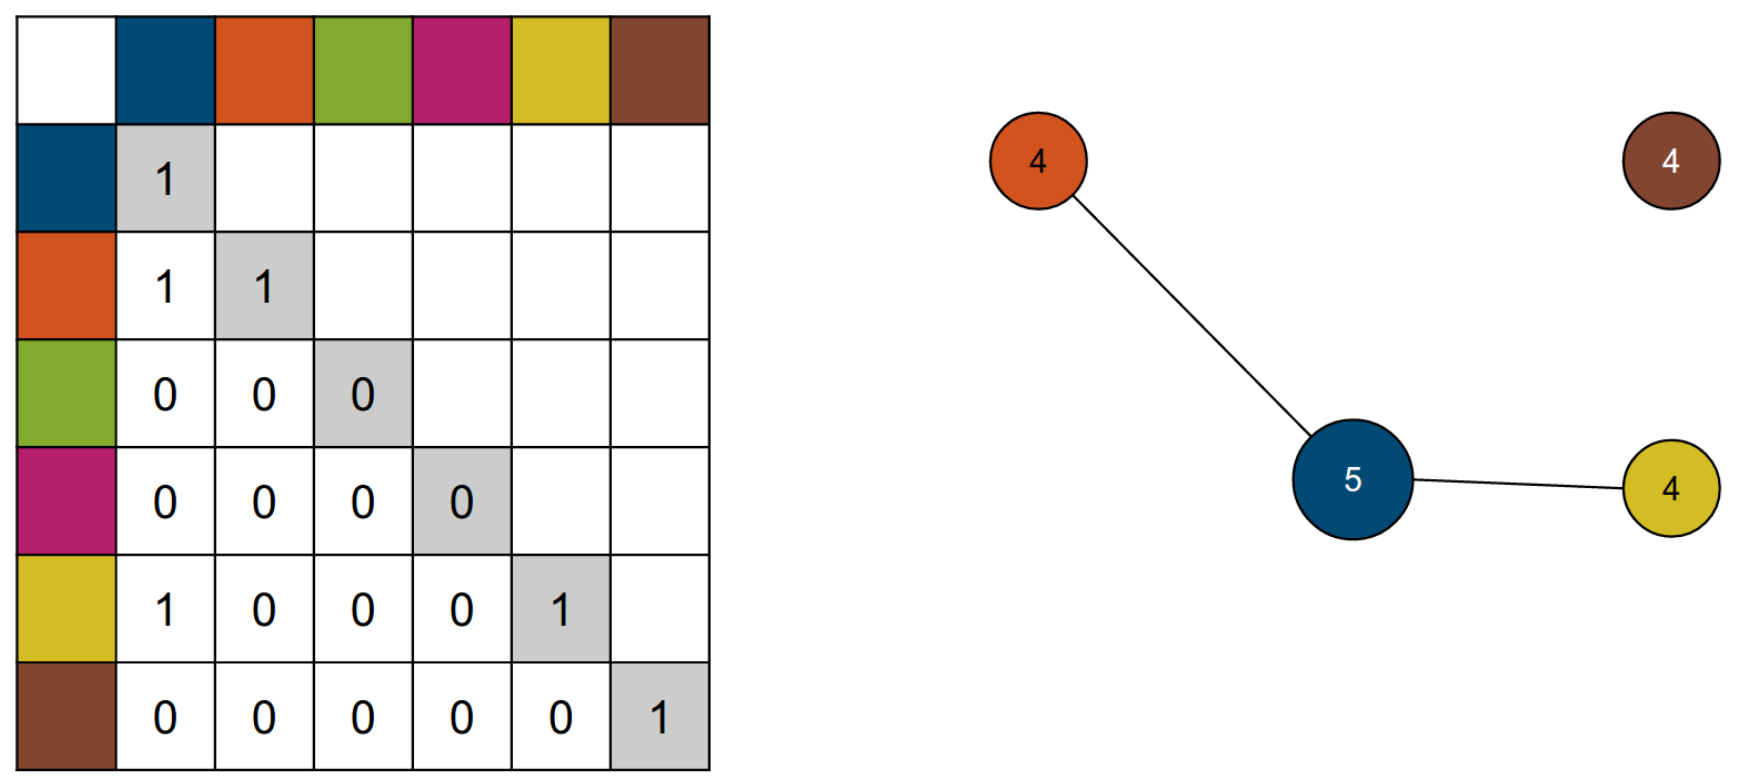
\includegraphics[width=0.8\textwidth]{img/matrixtrashed}
		\caption{This is the resulting clique graph after thresholding with $k=4$. All connected components represent a $k$-clique- community. There are two communities in this example.}
		\label{fig:matrixtrashed}
\end{center}
\end{figure}
 
\subsubsection{(4) Each connected component in the clique graph forms a $k$-clique- community.}
In the resulting graph, we need to look for connected components that represent the $k$-clique- communities, see Figure~\ref{fig:final}.

\subsubsection{(5) Post-processing.}
The last step of the algorithm assigns leftover nodes, if possible, to communities. A node which is only connected to one particular community and is not part of a community is associated with this community. The number of nodes belonging to a community can be increased.

\begin{figure}
\begin{center}
	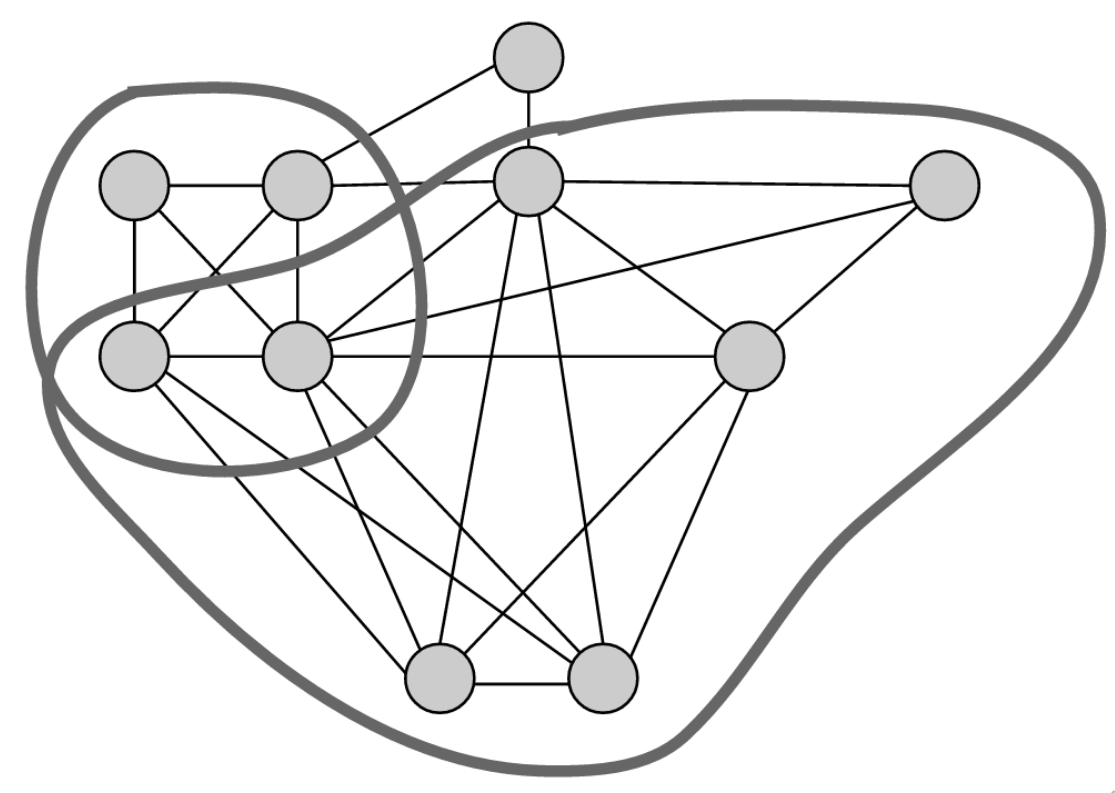
\includegraphics[width=0.8\textwidth]{img/final}
		\caption{Here the two resulting $k$-clique- communities are shown.}
		\label{fig:final}
\end{center}
\end{figure}


\subsection{Construction of the Co-Authorship Network}
\label{cpm-construction}
The edge weights are calculated with $$\frac{n}{n-1}$$, with $n$ being the number of authors per publication.
This leads to modelling the collaboration between fewer authors as more intensive than the collaboration between a higher number of authors.  
To generate an unweighted network, all edges with an edge weight below a certain threshold $w^*$ need to be removed. All other edge weights are replaced by weight $1$. Increasing $w^*$ results in fewer edges throughout the network, but stronger links and fewer detected communities.

Additionally, a good $k$ needs to be chosen. When $k$ is increased, the detected $k$-clique- communities shrink, but at the same time they become more cohesive (stronger connected).
So a good balance between $k$ and $w^*$ needs to be found to obtain a highly structured community.

The authors state that $k$ is usually between $3$ and $6$.
If the number of links in a network is increased above a certain point, a giant component evolves and covers the underlying community structure.
Therefore, for each $k$, the threshold $w^*$ is lowered until the largest component becomes twice as big as the second-largest component. To choose the best $k$, some further characteristics describing the community structure need to be investigated. See supplementary information of~\cite{palla2005uncovering} for more details.

\subsection{Main Findings of the Paper}
Overlaps in networks are significant. The distributions introduced in the paper (community size, community degree, overlap size, and membership number) reveal universal features of networks. The network of communities has non-trivial correlations and specific scaling properties.~\cite{palla2005uncovering}

\section{Community Evolution}
\label{evolution}
Palla et~al.~\cite{palla2007quantifying} developed an algorithm based on clique percolation (see Section~\ref{cpm}) that allows the investigation of overlapping communities over time. They uncovered basic relationships that characterize community evolution within a co-authorship network and a phone-call network. The following section describes the main steps of the algorithm. A short summary of their main findings can be found in Section~\ref{evolution-findings}.

\subsection{Algorithm}
\label{evolution-algo}
The starting point of the algorithm is an undirected and unweighted graph for each time step.
The construction of those temporal graphs is explained in Section~\ref{evolution-constr}.
In general, the algorithm uses the clique percolation method to find communities in each temporal graph, and subsequently matches the communities of consecutive time steps.

\medskip

\noindent
\colorbox{usethiscolorhere}{
\begin{minipage}{\dimexpr\textwidth-2\fboxsep}

\begin{enumerate}
\small
\item[(1)] Extract communities with CPM for each graph $g_t$ at time step $t$.
\item[(2)] Match set of communities at consecutive time steps of graph $g_t$, $g_{t+1}$, as follows:
	\begin{enumerate}
		\item[(2.1)] Construct joint graph $g_{\cup}=g_t \cup g_{t+1}$.
		\item[(2.2)] Extract communities $V$ with CPM in joint graph $g_{\cup}$.
		\item[(2.3)] For each extracted community $V_i$: 
		\begin{itemize}
			\item Extract communities in $g_t$ and $g_{t+1}$ that are contained in $V_i$.
			\item Calculate relative overlap for each pair.
			\item Match communities in descending order.
		\end{itemize}
	\end{enumerate}
\item[(3)] Post-processing.
\end{enumerate}

\end{minipage}
}

\medskip

The following section describes the steps (2) Matching Communities and (3) Post-Processing in detail.
Step (1) was already explained in Section~\ref{cpm}.

\subsubsection{Matching Communities}
\label{evolution-algo-matching}
For matching communities, the \emph{relative node overlap} $C(A,B)$ between the nodes $A$ and $B$, is defined simply as
$$C(A,B) = \frac{ \left| A \cap B\right| }{\left| A \cup B\right|}.$$
As overlapping communities are allowed, the matching from consecutive time steps in descending order of their relative node overlap can lead to mismatching, such as when small communities gain a lot of members or vice versa. An example for this problem is given in Figure~\ref{fig:mismatch}.
As a solution, for each of the time steps $t$ and $t+1$, a joint graph $g_{\cup}$ is constructed, that contains all links from both networks.
Let $D$ be the set of communities at time step $t$, and $E$ the set of communities at time step $t+1$. The set of communities from the joint graph $g_{\cup}$ are extracted using CPM and are called $V$.
For any community $D_i \in D$ or $E_j \in E$, exactly one community $V_k \in V$ can be found.
To check whether $E_i$ or $D_j$ is contained in $V_k$, the links are compared instead of nodes.
For each community $V_i \in V$, the sets of communities $D_i^k \in D$ and $E_j^k \in E$ contained in $V_i$ are extracted.
Now the relative node overlap between every possible pair can be calculated with
$$C^k_{i,j} = \frac{\left| D_i^k \cap E_j^k\right|}{\left| D_i^k\cup E_j^k \right| }$$
and the pairs can be matched in descending order.

\begin{figure}
\begin{center}
	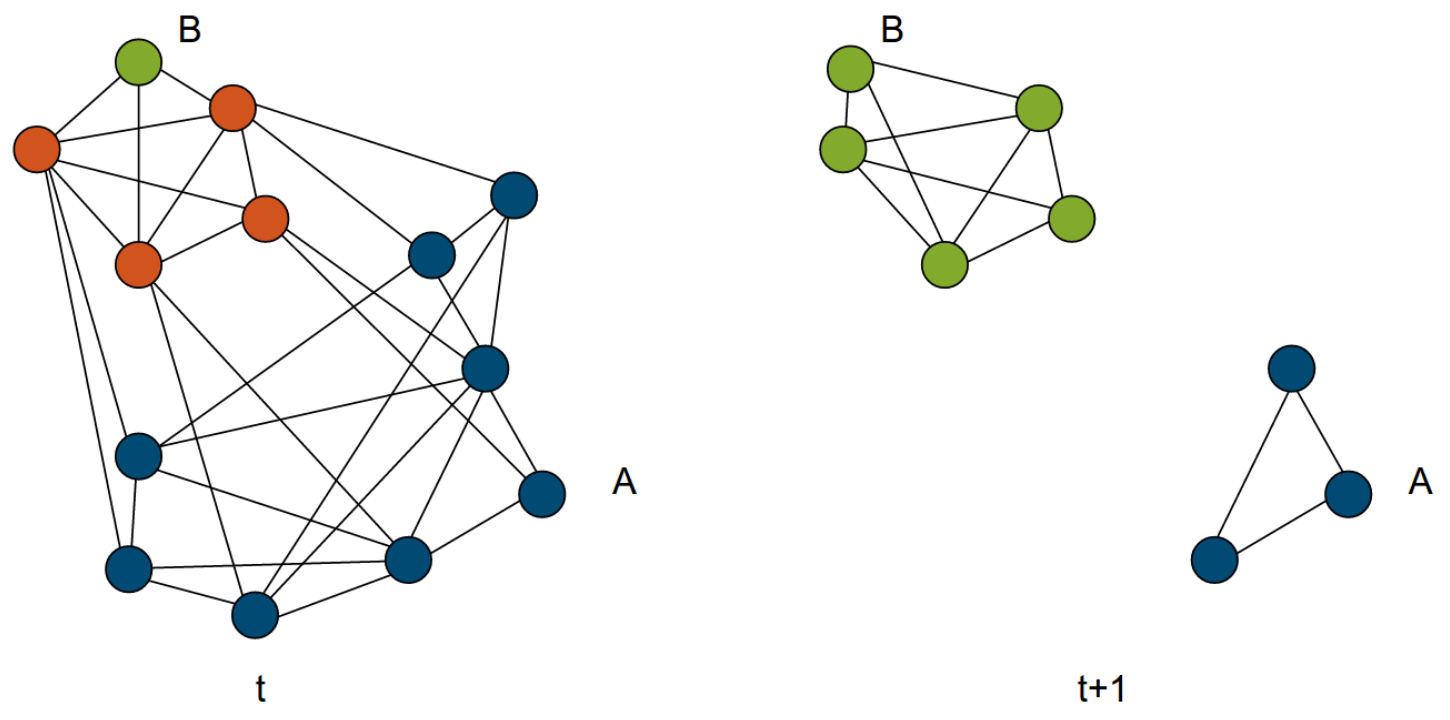
\includegraphics[width=0.8\textwidth]{img/mismatch.png}
		\caption{Example of mismatching communities in consecutive time steps. $A$(green) and $B$(blue) are two communities. Red nodes belong to both communities. The overlap between $A_t$ and $B_{t+1}$ is bigger than that between $A_t$ and $A_{t+1}$}.
		\label{fig:mismatch}
\end{center}
\end{figure}

\subsubsection{Post-Processing}
In some cases, a community that was disintegrated at a certain time step suddenly reappears in a later time step due to low publishing rates, for example.
This means a newborn community includes a dead community.
This problem is overcome by just filling the gap with the last step of the almost disintegrated community, which is called gap filling.

\subsection{Construction of the Temporal Co-Authorship Networks}
\label{evolution-constr}
Events in the co-authorship network are publications.
The social contract between people writing a paper together usually starts before the event and lasts for some time after the event. The higher the frequency, the closer the relationship~\cite{ramasco2006social}.

The edge weight resulting from one paper is $n/(n-1)$ with $n$ as the number of authors.
The edge weight between the nodes $a$ and $b$ at a certain time $t$ is calculated as

$$w_{a,b}(t)= \sum_{i}^{} w_i e^{\frac{-\lambda \left|t-t_i\right|}{w_i}}.$$

The summation runs over all collaborative events in which $a$ and $b$ are involved.
The event $i$ occurs at time $t_i$ and the corresponding edge weight at this time is called $w_i$.
Considerinh all events ever occurred in time, this decay function models the strength of the collaboration between authors over time.

A threshold $w^*$ is used to include only certain edges in the temporal graph. Hence, for each time step, a graph can be constructed based on the collaboration strength per time step.

The authors of the paper used $w^*=1.0$ for the co-authorship network.
The paper gives no details about $\lambda$.
The dataset used in the paper contained 142 months of publications. Details of data aggregation are not provided. However, with respect to figures, it appears to be 50 time slices.

\subsection{Main Findings of the Paper}
\label{evolution-findings}
The paper summarized differences between large and small communities and their development over time. Small communities live longer if their members remain unchanged over time. If members in small communities change frequently, they live only for a short time. Large communities live longer if members are changed permanently; if the members remain the same, they die quickly.

\section{Implications and Efficiency of the Algorithm}
This part describes the steps I would need to undertake to carry out a temporal analysis of communities within the geochemistry dataset or within any other dataset, that forms a collaboration network.

\medskip

\noindent
\colorbox{usethiscolorhere}{
\begin{minipage}{\dimexpr\textwidth-2\fboxsep}

\begin{enumerate}
\small
	\item[(1)] Generate slices of the network for each year.
	\item[(2)] Find function for calculating edge weights.
	\item[(3)] Apply edge weights to each snapshot.
	\item[(4)] Find out $k$.
	\item[(5)] Adjust threshold $w^*$ according to $k$.	
	\item[(6)] Do CPM for each snapshot.
	\item[(7)] Conduct community mapping.
\end{enumerate}

\end{minipage}
}

\medskip

It is necessary to evaluate the quality of the resulting network after step (1) time slicing, by looking at the basic statistics (number of publications per time slice, degree distribution, average nodes per time slice).
The function for calculating edge weights (2) could be taken from the paper (see Section~\ref{evolution-constr}), but it should be checked if the resulting networks after step (3) are still valid.
To find the right $k$ (4) and $w^*$ (5) the analysis of network characteristics like coverage of community structure and distribution if community size needs to be extended.
Moreover, the quality of the detected communities would need evaluation when the density within the community is compared to with outside the community.
For step (1), CFinder or R could be used.
I am open to the idea of implementation for the community mapping (7). If there were none, this step would need to be implemented.

Determining all cliques within a graph gives rise to a non-polynomial problem.
The authors state that the required CPU time largely depends on the structure of the input data, so no closed formula can be given to estimate the system size dependence.
A complete CPM analysis of a co-authorship network with $127.000$ links takes less than two hours on a PC\footnote{The paper provides no details about the PC.}.
I assume that time complexity will not be a problem as my dataset contains $18.404$ edges in total when no threshold is being applied.

\section{Future Work}
As this paper discusses only one popular method, an extensive literature research should follow, to check out more methods for solving the problem. In addition, a closer look at more recent work would be necessary. It would be equally interesting to come up with a good model for calculating edge weights with respect to the definition of scientific collaboration. The visualization of the community evolution, which remains open, would be a broad and exciting topic to investigate further.

{
	\bibliographystyle{plain}
	\bibliography{papers}
}



\end{document}
